% interactcadsample.tex
% v1.03 - April 2017

\documentclass[]{interact}

\usepackage{epstopdf}% To incorporate .eps illustrations using PDFLaTeX, etc.
\usepackage{subfigure}% Support for small, `sub' figures and tables
%\usepackage[nolists,tablesfirst]{endfloat}% To `separate' figures and tables from text if required

\usepackage{natbib}% Citation support using natbib.sty
\bibpunct[, ]{(}{)}{;}{a}{}{,}% Citation support using natbib.sty
\renewcommand\bibfont{\fontsize{10}{12}\selectfont}% Bibliography support using natbib.sty

\theoremstyle{plain}% Theorem-like structures provided by amsthm.sty
\newtheorem{theorem}{Theorem}[section]
\newtheorem{lemma}[theorem]{Lemma}
\newtheorem{corollary}[theorem]{Corollary}
\newtheorem{proposition}[theorem]{Proposition}

\theoremstyle{definition}
\newtheorem{definition}[theorem]{Definition}
\newtheorem{example}[theorem]{Example}

\theoremstyle{remark}
\newtheorem{remark}{Remark}
\newtheorem{notation}{Notation}

% see https://stackoverflow.com/a/47122900
\usepackage{color}
\usepackage{fancyvrb}
\newcommand{\VerbBar}{|}
\newcommand{\VERB}{\Verb[commandchars=\\\{\}]}
\DefineVerbatimEnvironment{Highlighting}{Verbatim}{commandchars=\\\{\}}
% Add ',fontsize=\small' for more characters per line
\usepackage{framed}
\definecolor{shadecolor}{RGB}{248,248,248}
\newenvironment{Shaded}{\begin{snugshade}}{\end{snugshade}}
\newcommand{\AlertTok}[1]{\textcolor[rgb]{0.94,0.16,0.16}{#1}}
\newcommand{\AnnotationTok}[1]{\textcolor[rgb]{0.56,0.35,0.01}{\textbf{\textit{#1}}}}
\newcommand{\AttributeTok}[1]{\textcolor[rgb]{0.77,0.63,0.00}{#1}}
\newcommand{\BaseNTok}[1]{\textcolor[rgb]{0.00,0.00,0.81}{#1}}
\newcommand{\BuiltInTok}[1]{#1}
\newcommand{\CharTok}[1]{\textcolor[rgb]{0.31,0.60,0.02}{#1}}
\newcommand{\CommentTok}[1]{\textcolor[rgb]{0.56,0.35,0.01}{\textit{#1}}}
\newcommand{\CommentVarTok}[1]{\textcolor[rgb]{0.56,0.35,0.01}{\textbf{\textit{#1}}}}
\newcommand{\ConstantTok}[1]{\textcolor[rgb]{0.00,0.00,0.00}{#1}}
\newcommand{\ControlFlowTok}[1]{\textcolor[rgb]{0.13,0.29,0.53}{\textbf{#1}}}
\newcommand{\DataTypeTok}[1]{\textcolor[rgb]{0.13,0.29,0.53}{#1}}
\newcommand{\DecValTok}[1]{\textcolor[rgb]{0.00,0.00,0.81}{#1}}
\newcommand{\DocumentationTok}[1]{\textcolor[rgb]{0.56,0.35,0.01}{\textbf{\textit{#1}}}}
\newcommand{\ErrorTok}[1]{\textcolor[rgb]{0.64,0.00,0.00}{\textbf{#1}}}
\newcommand{\ExtensionTok}[1]{#1}
\newcommand{\FloatTok}[1]{\textcolor[rgb]{0.00,0.00,0.81}{#1}}
\newcommand{\FunctionTok}[1]{\textcolor[rgb]{0.00,0.00,0.00}{#1}}
\newcommand{\ImportTok}[1]{#1}
\newcommand{\InformationTok}[1]{\textcolor[rgb]{0.56,0.35,0.01}{\textbf{\textit{#1}}}}
\newcommand{\KeywordTok}[1]{\textcolor[rgb]{0.13,0.29,0.53}{\textbf{#1}}}
\newcommand{\NormalTok}[1]{#1}
\newcommand{\OperatorTok}[1]{\textcolor[rgb]{0.81,0.36,0.00}{\textbf{#1}}}
\newcommand{\OtherTok}[1]{\textcolor[rgb]{0.56,0.35,0.01}{#1}}
\newcommand{\PreprocessorTok}[1]{\textcolor[rgb]{0.56,0.35,0.01}{\textit{#1}}}
\newcommand{\RegionMarkerTok}[1]{#1}
\newcommand{\SpecialCharTok}[1]{\textcolor[rgb]{0.00,0.00,0.00}{#1}}
\newcommand{\SpecialStringTok}[1]{\textcolor[rgb]{0.31,0.60,0.02}{#1}}
\newcommand{\StringTok}[1]{\textcolor[rgb]{0.31,0.60,0.02}{#1}}
\newcommand{\VariableTok}[1]{\textcolor[rgb]{0.00,0.00,0.00}{#1}}
\newcommand{\VerbatimStringTok}[1]{\textcolor[rgb]{0.31,0.60,0.02}{#1}}
\newcommand{\WarningTok}[1]{\textcolor[rgb]{0.56,0.35,0.01}{\textbf{\textit{#1}}}}

% Pandoc citation processing

\usepackage{hyperref}
\usepackage[utf8]{inputenc}
\def\tightlist{}


\begin{document}

\articletype{ARTICLE TEMPLATE}

\title{External Validation of Berten's Model for Predicting COPD
Exacerbations}


\author{\name{Amin Adibi$^{a}$, Don Sin$^{b}$, Mohsen Sadatsafavi$^{a,
\dagger, \ddagger}$}
\affil{$^{a}$Respiratory Evaluation Sciences Program, Faculty of
Pharmaceutical Sciences, University of British Columbia, Vancouver, BC,
Canada; $^{b}$Division of Respiratory Medicine, Department of Medicine,
The UBC Centre for Heart Lung Innovation, St.~Paul's Hospital,
University of British Columbia, Vancouver, BC, Canada}
}

\thanks{CONTACT Amin
Adibi. Email: \href{mailto:amin.adibi@ubc.ca}{\nolinkurl{amin.adibi@ubc.ca}}, Don
Sin. Email: \href{mailto:don.sin@hli.ubc.ca}{\nolinkurl{don.sin@hli.ubc.ca}}, Mohsen
Sadatsafavi. Email: \href{mailto:mohsen.sadatsafavi@ubc.ca}{\nolinkurl{mohsen.sadatsafavi@ubc.ca}}}

\maketitle

\begin{abstract}
We are reporting an independent validation of the COPD exacerbation
prediction model developed by Bertens and colleagues in the
\end{abstract}

\begin{keywords}
COPD; prediction; validation
\end{keywords}

\hypertarget{introduction}{%
\section{Introduction}\label{introduction}}

The Berten's model \citep{bertens_development_2013}.

\hypertarget{methods}{%
\section{Methods}\label{methods}}

We have followed recommendations of the Transparent Reporting of a
Multivariable Prediction Model for Individual Prognosis or Diagnosis
(the TRIPOD Statement) \citep{collins_transparent_2015} in reporting our
independent validation of the Bertens model. External validation was
done using three years of data from COPD patients enrolled in the
Evaluation of COPD Longitudinally to Identify Predictive Surrogate
End-points (the ECLIPSE Study), an independent non-interventional
observational longitudinal COPD cohort study that was aimed at
characterizing progression of the
disease\citep{agusti_characterisation_2010}.

The first year of the ECLIPSE study was used to establish exacerbation
history, year two was used to assess validity of one-year and two-year
predictions were assessed using data from year two, and years 2-3,
respectively.

We report external validation of the model in terms of calibration (the
degree to which predicted and observed risk of exacerbations are in
agreement), discrimination (the extend to which the model is able to
separate higher and lower risk individuals), and clinical utility (net
benefit across different risk thresholds for treatment decision).

Calibration was assessed through visual examination of the calibration
curve. Differentiation was assessed by plotting the Receiver Operating
Characteristic (ROC) curve and its area-under-the-curve (AUC), also
known as the c-statistic. Clinical utility was assesses through have
reported Decision Curve Analysis \citep{vickers_simple_2019}.

The study was approved by the University of British Columbia and
Providence Health Research Ethics Board (H11--00786).

\hypertarget{results}{%
\section{Results}\label{results}}

\hypertarget{discsussions}{%
\section{Discsussions}\label{discsussions}}

\hypertarget{code-chunks}{%
\subsection{Code chunks}\label{code-chunks}}

\hypertarget{including-plots}{%
\subsection{Including Plots}\label{including-plots}}

You can also embed plots, for example:

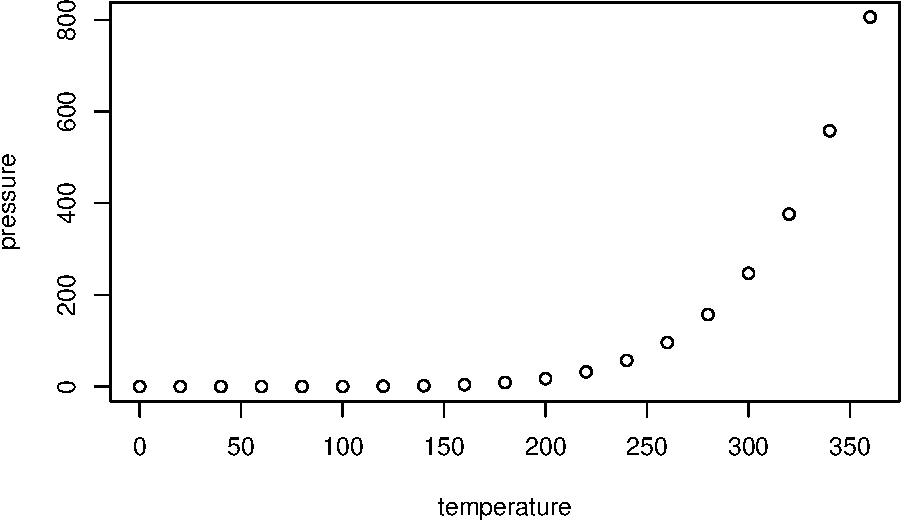
\includegraphics[width=0.8\linewidth]{External-Validation-of-Bertens-COPD-Exacebration-Model_files/figure-latex/pressure-1}

Note that the \texttt{echo\ =\ FALSE} parameter was added to the code
chunk to prevent printing of the R code that generated the plot.

\hypertarget{some-guidelines-for-using-the-standard-features-of}{%
\section{\texorpdfstring{Some guidelines for using the standard features
of
\LaTeX}{Some guidelines for using the standard features of }}\label{some-guidelines-for-using-the-standard-features-of}}

\hypertarget{sections}{%
\subsection{Sections}\label{sections}}

The \textsf{Interact} layout style allows for five levels of section
heading, all of which are provided in the \texttt{interact} class file
using the standard \LaTeX~commands \texttt{\textbackslash{}section},
\texttt{\textbackslash{}subsection},
\texttt{\textbackslash{}subsubsection},
\texttt{\textbackslash{}paragraph} and
\texttt{\textbackslash{}subparagraph}. Numbering will be automatically
generated for all these headings by default.

\hypertarget{lists}{%
\subsection{Lists}\label{lists}}

Numbered lists are produced using the \texttt{enumerate} environment,
which will number each list item with arabic numerals by default. For
example,

\begin{enumerate}
\def\labelenumi{\arabic{enumi}.}
\tightlist
\item
  first item
\item
  second item
\item
  third item
\end{enumerate}

Alternative numbering styles can be achieved by inserting an optional
argument in square brackets to each \texttt{item},
e.g.~\texttt{\textbackslash{}item{[}(i){]}\ first\ item}, to create a
list numbered with roman numerals at level one.

Bulleted lists are produced using the \texttt{itemize} environment. For
example,

\begin{itemize}
\tightlist
\item
  First bulleted item
\item
  Second bulleted item
\item
  Third bulleted item
\end{itemize}

\hypertarget{figures}{%
\subsection{Figures}\label{figures}}

\begin{Shaded}
\begin{Highlighting}[]
\FunctionTok{plot}\NormalTok{(pressure)}
\end{Highlighting}
\end{Shaded}

The \texttt{interact} class file will deal with positioning your figures
in the same way as standard \LaTeX. It should not normally be necessary
to use the optional \texttt{{[}htb{]}} location specifiers of the
\texttt{figure} environment in your manuscript; you may, however, find
the \texttt{{[}p{]}} placement option or the \texttt{endfloat} package
useful if a journal insists on the need to separate figures from the
text.

Figure captions appear below the figures themselves, therefore the
\texttt{\textbackslash{}caption} command should appear after the body of
the figure. For example, Figure\textasciitilde{}\ref{sample-figure} with
caption and sub-captions is produced using the following commands:

\begin{verbatim}
\begin{figure}
\centering
\subfigure[An example of an individual figure sub-caption.]{%
\resizebox*{5cm}{!}{\includegraphics{path/to/fig}}}\hspace{5pt}
\subfigure[A slightly shorter sub-caption.]{%
\resizebox*{5cm}{!}{\includegraphics{path/to/fig}}}
\caption{Example of a two-part figure with individual sub-captions
 showing that captions are flush left and justified if greater
 than one line of text.} \label{sample-figure}
\end{figure}
\end{verbatim}

\begin{figure}
\centering
\subfigure[An example of an individual figure sub-caption.]{%
\resizebox*{5cm}{!}{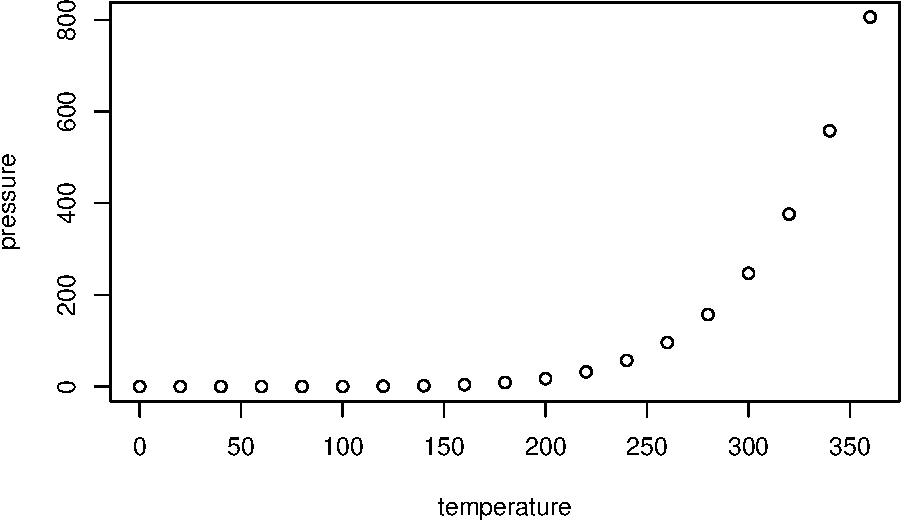
\includegraphics{External-Validation-of-Bertens-COPD-Exacebration-Model_files/figure-latex/pressure-plot-1.pdf}}}\hspace{5pt}
\subfigure[A slightly shorter sub-caption.]{%
\resizebox*{5cm}{!}{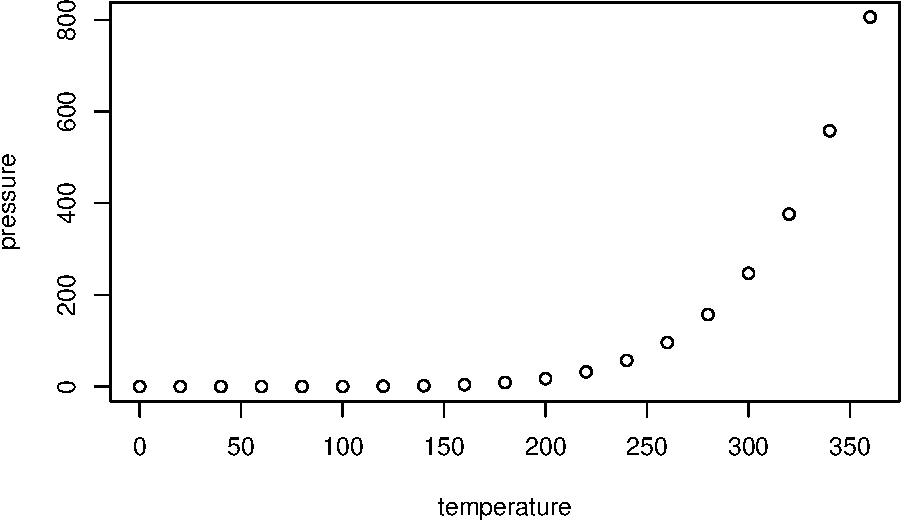
\includegraphics{External-Validation-of-Bertens-COPD-Exacebration-Model_files/figure-latex/pressure-plot-1.pdf}}}
\caption{Example of a two-part figure with individual sub-captions
 showing that captions are flush left and justified if greater
 than one line of text.} \label{sample-figure}
\end{figure}

To ensure that figures are correctly numbered automatically, the
\texttt{\textbackslash{}label} command should be included just after the
\texttt{\textbackslash{}caption} command, or in its argument.

The \texttt{\textbackslash{}subfigure} command requires
\texttt{subfigure.sty}, which is called in the preamble of the
\texttt{interacttfssample.tex} file (to allow your choice of an
alternative package if preferred) and included in the \textsf{Interact}
\LaTeX~bundle for convenience. Please supply any additional figure
macros used with your article in the preamble of your .tex file.

The source files of any figures will be required when the final, revised
version of a manuscript is submitted. Authors should ensure that these
are suitable (in terms of lettering size, etc.) for the reductions they
envisage.

The \texttt{epstopdf} package can be used to incorporate encapsulated
PostScript (.eps) illustrations when using PDF\LaTeX, etc. Please
provide the original .eps source files rather than the generated PDF
images of those illustrations for production purposes.

\hypertarget{tables}{%
\subsection{Tables}\label{tables}}

The \texttt{interact} class file will deal with positioning your tables
in the same way as standard \LaTeX. It should not normally be necessary
to use the optional \texttt{{[}htb{]}} location specifiers of the
\texttt{table} environment in your manuscript; you may, however, find
the \texttt{{[}p{]}} placement option or the \texttt{endfloat} package
useful if a journal insists on the need to separate tables from the
text.

The \texttt{tabular} environment can be used as shown to create tables
with single horizontal rules at the head, foot and elsewhere as
appropriate. The captions appear above the tables in the
\textsf{Interact} style, therefore the \texttt{\textbackslash{}tbl}
command should be used before the body of the table. For example,
Table\textasciitilde{}\ref{sample-table} is produced using the following
commands:

\begin{table}
\tbl{Example of a table showing that its caption is as wide as
 the table itself and justified.}
{\begin{tabular}{lcccccc} \toprule
 & \multicolumn{2}{l}{Type} \\ \cmidrule{2-7}
 Class & One & Two & Three & Four & Five & Six \\ \midrule
 Alpha\textsuperscript{a} & A1 & A2 & A3 & A4 & A5 & A6 \\
 Beta & B2 & B2 & B3 & B4 & B5 & B6 \\
 Gamma & C2 & C2 & C3 & C4 & C5 & C6 \\ \bottomrule
\end{tabular}}
\tabnote{\textsuperscript{a}This footnote shows how to include
 footnotes to a table if required.}
\label{sample-table}
\end{table}

\begin{verbatim}
\begin{table}
\tbl{Example of a table showing that its caption is as wide as
 the table itself and justified.}
{\begin{tabular}{lcccccc} \toprule
 & \multicolumn{2}{l}{Type} \\ \cmidrule{2-7}
 Class & One & Two & Three & Four & Five & Six \\ \midrule
 Alpha\textsuperscript{a} & A1 & A2 & A3 & A4 & A5 & A6 \\
 Beta & B2 & B2 & B3 & B4 & B5 & B6 \\
 Gamma & C2 & C2 & C3 & C4 & C5 & C6 \\ \bottomrule
\end{tabular}}
\tabnote{\textsuperscript{a}This footnote shows how to include
 footnotes to a table if required.}
\label{sample-table}
\end{table}
\end{verbatim}

To ensure that tables are correctly numbered automatically, the
\texttt{\textbackslash{}label} command should be included just before
\texttt{\textbackslash{}end\{table\}}.

The \texttt{\textbackslash{}toprule}, \texttt{\textbackslash{}midrule},
\texttt{\textbackslash{}bottomrule} and
\texttt{\textbackslash{}cmidrule} commands are those used by
\texttt{booktabs.sty}, which is called by the \texttt{interact} class
file and included in the \textsf{Interact} \LaTeX~bundle for
convenience. Tables produced using the standard commands of the
\texttt{tabular} environment are also compatible with the
\texttt{interact} class file.

\hypertarget{landscape-pages}{%
\subsection{Landscape pages}\label{landscape-pages}}

If a figure or table is too wide to fit the page it will need to be
rotated, along with its caption, through 90\(^{\circ}\) anticlockwise.
Landscape figures and tables can be produced using the \texttt{rotating}
package, which is called by the \texttt{interact} class file. The
following commands (for example) can be used to produce such pages.

\begin{verbatim}
\setcounter{figure}{1}
\begin{sidewaysfigure}
\centerline{\epsfbox{figname.eps}}
\caption{Example landscape figure caption.}
\label{landfig}
\end{sidewaysfigure}
\end{verbatim}

\begin{verbatim}
\setcounter{table}{1}
\begin{sidewaystable}
 \tbl{Example landscape table caption.}
  {\begin{tabular}{@{}llllcll}
    .
    .
    .
  \end{tabular}}\label{landtab}
\end{sidewaystable}
\end{verbatim}

Before any such float environment, use the
\texttt{\textbackslash{}setcounter} command as above to fix the
numbering of the caption (the value of the counter being the number
given to the preceding figure or table). Subsequent captions will then
be automatically renumbered accordingly. The
\texttt{\textbackslash{}epsfbox} command requires \texttt{epsfig.sty},
which is called by the \texttt{interact} class file and is also included
in the \textsf{Interact} \LaTeX~bundle for convenience.

Please note that if the \texttt{endfloat} package is used, one or both
of the commands

\begin{verbatim}
\DeclareDelayedFloatFlavor{sidewaysfigure}{figure}
\DeclareDelayedFloatFlavor{sidewaystable}{table}
\end{verbatim}

will need to be included in the preamble of your .tex file, after the
\texttt{endfloat} package is loaded, in order to process any landscape
figures and/or tables correctly.

\hypertarget{acknowledgements}{%
\section*{Acknowledgement(s)}\label{acknowledgements}}
\addcontentsline{toc}{section}{Acknowledgement(s)}

An unnumbered section,
e.g.~\texttt{\textbackslash{}section*\{Acknowledgements\}}, may be used
for thanks, etc.~if required and included \emph{in the non-anonymous
version} before any Notes or References.

\hypertarget{disclosure-statement}{%
\section*{Disclosure statement}\label{disclosure-statement}}
\addcontentsline{toc}{section}{Disclosure statement}

An unnumbered section,
e.g.~\texttt{\textbackslash{}section*\{Disclosure\ statement\}}, may be
used to declare any potential conflict of interest and included \emph{in
the non-anonymous version} before any Notes or References, after any
Acknowledgements and before any Funding information.

\hypertarget{funding}{%
\section*{Funding}\label{funding}}
\addcontentsline{toc}{section}{Funding}

An unnumbered section,
e.g.~\texttt{\textbackslash{}section*\{Funding\}}, may be used for grant
details, etc.~if required and included \emph{in the non-anonymous
version} before any Notes or References.

\hypertarget{notes-on-contributors}{%
\section*{Notes on contributor(s)}\label{notes-on-contributors}}
\addcontentsline{toc}{section}{Notes on contributor(s)}

An unnumbered section,
e.g.~\texttt{\textbackslash{}section*\{Notes\ on\ contributors\}}, may
be included \emph{in the non-anonymous version} if required. A
photograph may be added if requested.

\hypertarget{nomenclaturenotation}{%
\section*{Nomenclature/Notation}\label{nomenclaturenotation}}
\addcontentsline{toc}{section}{Nomenclature/Notation}

An unnumbered section,
e.g.~\texttt{\textbackslash{}section*\{Nomenclature\}} (or
\texttt{\textbackslash{}section*\{Notation\}}), may be included if
required, before any Notes or References.

\hypertarget{notes}{%
\section*{Notes}\label{notes}}
\addcontentsline{toc}{section}{Notes}

An unnumbered \texttt{Notes} section may be included before the
References (if using the \texttt{endnotes} package, use the command
\texttt{\textbackslash{}theendnotes} where the notes are to appear,
instead of creating a \texttt{\textbackslash{}section*}).

\hypertarget{references}{%
\section{References}\label{references}}

\hypertarget{references-cited-in-the-text}{%
\subsection{References cited in the
text}\label{references-cited-in-the-text}}

\hypertarget{the-list-of-references}{%
\subsection{The list of references}\label{the-list-of-references}}

References should be listed at the end of the main text in alphabetical
order by authors' surnames, then chronologically (earliest first). If
references have the same author(s), editor(s), etc., arrange by year of
publication, with undated works at the end. A single-author entry
precedes a multi-author entry that begins with the same name. If the
reference list contains two or more items by the same author(s) in the
same year, add a, b, etc. and list them alphabetically by title.
Successive entries by two or more authors when only the first author is
the same are alphabetized by co-authors' surnames. If a reference has
more than ten named authors, list only the first seven, followed by `et
al.'. If a reference has no author or editor, order by title; if a date
of publication is impossible to find, use `n.d.' in its place.

The following list shows some sample references prepared in the Taylor
\& Francis Chicago author-date style.

\citep{Ade09, Alb05}

\bibliographystyle{tfcad}
\bibliography{RESP.bib}


\input{"appendix.tex"}


\end{document}
